% LaTeX Template for Project Report, Version 1.0

% Created by: Kakooza Allan Klaus
% 216007552
% CoCIS
% Contact Info: kkallan07@gmail.com

\documentclass[12pt, a4paper]{report}
\usepackage{acronym}
\usepackage[pdftex]{graphicx} %for embedding images
\usepackage{url} %for proper url entries
\usepackage[acronym]{glossaries}
\usepackage{rotating}
\usepackage{amssymb}
\setcounter{tocdepth}{4}
\setcounter{secnumdepth}{4}
\usepackage{multido}
\usepackage{amssymb}
\usepackage{pifont}

\newcommand{\Pointilles}[1]{%
  \par\nobreak
  \noindent\rule{0pt}{1.0\baselineskip}% Provides a larger gap between the preceding paragraph and the dots
  \multido{}{#1}{\noindent\makebox[\linewidth]{\dotfill}\endgraf}% ... dotted lines ...
  \bigskip% Gap between dots and next paragraph
}

\usepackage{enumitem,amssymb}
\newlist{todolist}{itemize}{2}
\setlist[todolist]{label=$\square$}

\usepackage{tabularx,ragged2e,booktabs,caption}

\newcommand{\cmark}{\ding{51}}
\newcommand{\xmark}{\ding{55}}
\newcommand{\quotes}[1]{``#1''}


\begin{document}
\renewcommand\bibname{References} %Renames "Bibliography" to "References" on ref page

\pagenumbering{roman} %numbering before main content starts
%Include first stuff: title, acknowledgement, dedication, tables, etc
\begin{titlepage}

\begin{center}


\includegraphics[width=1\textwidth]{img/maklogo}\\%\\[0.1in]
\vspace{3em}%
% Title
\Large {A REPORT ON}\\%\\[0.5in]
\Large{FIELD ATTACHMENT/INTERNSHIP AT}\\
\normalsize Banana Phone World \\%
\vspace{1em}%
\normalsize 05/June/2018 - 02/August/2018 \\
\normalsize BY \\%
\vspace{1em}
\textup{\small {\bf Kakooza Allan Klaus}\\}
\textup{\small {\bf 16/U/5230/EVE}\\}
 \vspace{1em}%

\emph{Field Attachment Report submitted to the School of Computing and Informatics Technology or\\College of Computing and Information Sciences.\\
In Partial fulfillment of the requirements for the degree of (state your programme) of Makerere \\University Kampala.}

       % \small \emph{Submitted in partial fulfillment of\\
       %  the requirements for the award of the degree of}
        \vspace{1in}

       

% Submitted by
\raggedright {\bf Name \& Sign of Field Supervisor:...............................................} 
\begin{flushright}
\small{(Stamp \& Date)}
\end{flushright}



\raggedright{\bf Name \& Sign of Academic Supervisor:........................................} 
\begin{flushright}
\small{(Date)}
\end{flushright}


% {\textbf{<Guide's name here>}}\\[0.2in]

\vfill



\end{center}

\end{titlepage}

\cleardoublepage
\addcontentsline{toc}{chapter}{Declaration}
\chapter*{Declaration}
I Kakooza Allan Klaus do hereby declare that this Internship Report is original and has not been published and/or submitted for any other degree award to any other University before.


\vspace{1.0in}

\newpage


\cleardoublepage
\addcontentsline{toc}{chapter}{Acknowledgement}
\chapter*{Acknowledgement}


\noindent I am very appreciated to Mr. Sewanonda Dagan, my supervisor at Banana Phone World. Dagan gave me very in-time valuable instructions and put me in contact with experts in the field like Mr.
Alex Onyango, Value Added Services Manager at MTN, who gave me extensive guidance regarding many practical issues. I also would like to express my gratitude to Mr. Emmanuel Lule  for his permission to be my academic supervisor. \medskip

\noindent Throughout the internship, I have also learnt many things about the Chinese culture whose
benefits are far beyond what I could learn in a normal project. In short, I would like to thank
Banana Phone World and Makerere University, Internship Office especially Ms. Barbra Nansamba  for introducing me to this great opportunity in which I have developed myself both academically, professionally and socially.


\newpage




\cleardoublepage
\addcontentsline{toc}{chapter}{Abstract}
\chapter*{Abstract}
For three months from June 2018 till August 2018, I did my internship at Banana Phone World, a
phone distribution company which covers large areas in Uganda. Banana Phone World core
business involves distributing phones to a huge amount of customers which is
about nearly a fifth of Uganda's population. This internship project is a part of my Second
year program which I conduct at Makerere University of Uganda. \medskip.

\newpage







% \tableofcontents
% \input{./certificate.tex}
% \cleardoublepage
\addcontentsline{toc}{chapter}{Abstract}
\chapter*{Abstract}
For three months from June 2018 till August 2018, I did my internship at Banana Phone World, a
phone distribution company which covers large areas in Uganda. Banana Phone World core
business involves distributing phones to a huge amount of customers which is
about nearly a fifth of Uganda's population. This internship project is a part of my Second
year program which I conduct at Makerere University of Uganda. \medskip.

\newpage






\tableofcontents
\listoffigures
\listoftables

\cleardoublepage
\addcontentsline{toc}{chapter}{Abbreviations/Acronyms}
\chapter*{List of acronyms}

\begin{acronym}
  \acro{BPW}{Banana Phone World}
  \acro{IT}{Information Technology}
  \acro{FAQs}{Frequently asked Questions}
  \acro{PCB}{Printed Ciruit Board}
  \acro{GSM}{Global System for Mobile Communications}
  \acro{CDMA}{Code Division Multiple Access}
  \acro{PFO}{Power Frequency Oscillator}
  \acro{RF}{Radio Frequency}
  \acro{IC}{Integrated Circuit}
  \acro{CPU}{Central Processing Unit}
  \acro{MHz}{Mega Hertz}
  \acro{VCO}{Voltage-Controlled Oscillator}
  \acro{RX}{Receive / Receiver (Receiving Section)}
  \acro{TX}{Transmit (Transmitting Section)}
  \acro{ROM}{Read Only Memory}
  \acro{RAM}{Random Access Memory}
  \acro{RTC}{Real Time Clock}
  \acro{NGO}{Non-Government Organsation}
  \acro{SEO}{Search Engine Optimisation}
\end{acronym}

\newpage















\newpage
\pagenumbering{arabic} %reset numbering to normal for the main content

% \input{./prob-definition.tex} %objective changed to problem definition

\chapter{Introduction}
%
\includegraphics[width=1\textwidth]{img/BananaImage}\\%\\[0.1in]
%
\includegraphics[width=1in]{img/BananaImage}
The following report describes the activities carried out during my full­time internship at Banana Phone World (BPW) IT department. The report contains information about BPW IT department and the responsibilities performed throughout the training. Followed by the activities carried in this period and the projects worked on. It also addresses the experiences and challenges during this period. Finally, the report wraps up with a few closing recommendations and conclusions from the experience. 	

\section{Background}
\normalsize{\bf BPW} is a chinese company that was started on 22nd-06-2013 in Uganda, it deals in selling Tecno,Infinix and Itel phones both Smartphones and Features phones.They have 56 outlets across the country and they are still growing.\\ \\
It has 5 departments namely; Department of finance and administration (F\&A), Sales department, e-sales department(Egatee), IT department, Human Resource Department.\\ \\
The IT department has been successful in delivering services to the users, mainly end user support, technological innovations and solving IT technical problems. IT department has a team of technical experts both in Uganda and China whose goals are to offer solutions that tend to be complex in a simplified manner. Our consulting and integration of professionals provides the necessary expertise, experience and relationships to deliver customized solutions to users in the Banana Phone World to succeed today and tomorrow.

\begin{figure}
\centering
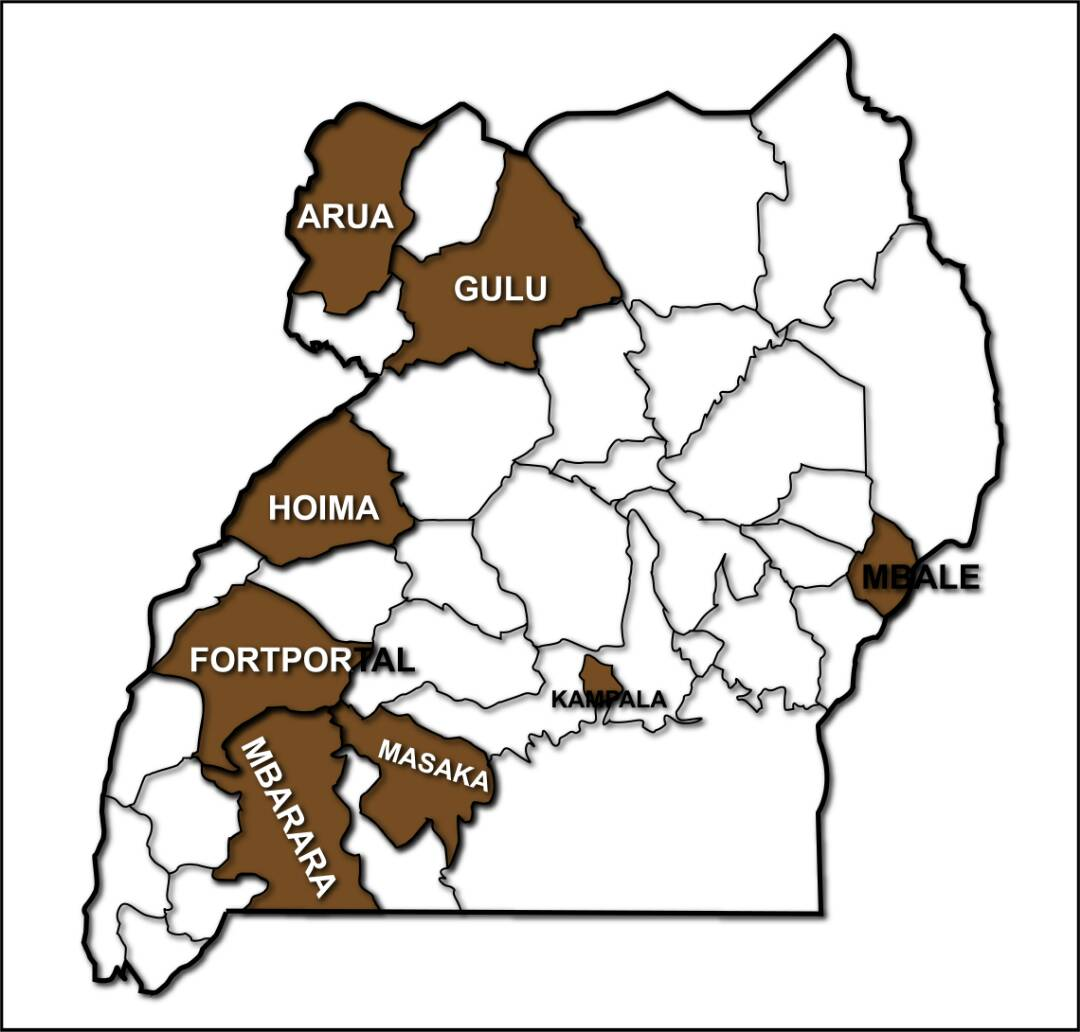
\includegraphics[width=2in]{img/Map}
\caption{Areas covered by BPW}
\end{figure}

\newpage
\subsection{Vision}
We exist to help our customers get the full benefit of communications services in their
daily lives. We want to make it easy for customers to get what they want, when they want it.
We're here to help.\\ \\
\normalsize {\bf Core Values}.
\begin{itemize}
\item	\textbf{Keep Promises:} Everything we set out to do should work, or if you don't get it, we’re here to help. We’re about delivery, not over promising actions not words. 
\item	\textbf{Be Inspiring:} We are creative. We strive to bring energy into the things we do. We produce should look good, modern and fresh. We are passionate about our business and customers. 
\item	\textbf{Be Respectful:} We acknowledge and respect local cultures. We do not impose formula worldwide. We want to be a part of local communities wherever we operate. We believe loyalty has to be earned.
\item	\textbf{Make It Easy:} We’re practical. We don't over complicate things. Everything we should be easy to understand and use. No waste. No jargon. Because we never forget we're trying to make customers' lives easier. 
\end{itemize}

\subsection{Mission}
Leading the industry and exceed customer expectations by providing the best phone services,
making life and business easier.

\subsection{Objective of Banana Phone World Ltd }
BPW basic strategy is coverage of both urban and rural areas. The Company has devised its strategies so that it earns healthy returns for its shareholders and at the same time, contributes to genuine development of the country. In short, it pursues a dual strategy of “Good Business, Good Development. Serving the mass market is one of GP's primary goals. By serving the general public as opposed to niche markets, the Company plans to achieve economies of scale and healthy profits.

\section{The Structure of the Organisation}

\begin{figure}[h!]
\begin{center}
	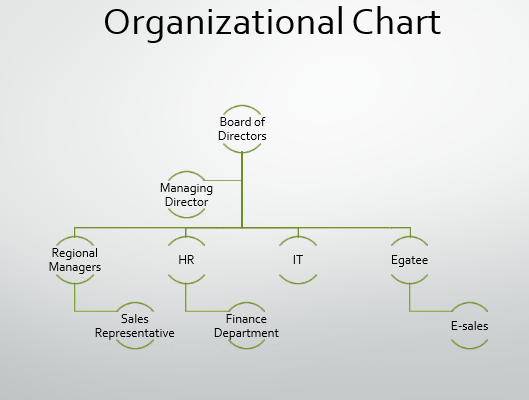
\includegraphics[scale=0.9]{img/Chart.PNG}
	\caption{Organisational Structure of BPW.}
	\label{fig:symbols}
\end{center}
\end{figure}


\section{The main activities of the organisation and ongoing activities IT projects}
\subsection{Main Activities Offered by the IT Department} 
\medskip
\begin{itemize}
\item Maintenance and hardware repairs services.
\item Power solutions. 
\item Testing, trouble shooting and repairs.
\item User Training.
\item Upgrades of systems and maintenance.
\item Manage accounts and passwords.
\item Email services.
\item Digital Marketing(Online Marketing).
\item Configuration management services.
\item Software Installations.
\end{itemize}
\subsection{Ongoing IT projects}
Banana Phone World Ltd is planning to bring in a system on board where you just swipe in your employee card an it marks the time you have arrived. %literature survey included in this
\chapter{Field Attachment Activities}
During my internship training at BPW, I did a number of activities such as Computer and Phone hardware maintenance, Software installations of operating systems and Drivers of all devices which were missing on computers and making updates, anti­viruses (Kaspersky installations), Installation and replacement of faulty components, Troubleshooting networks and computer hardware components, Digital Marketing\cite{Digital} etc. \\
During this period, I was able to gain more experience in this field of IT and add on my skills, improve on my socializing and interpersonal skills. 
\section{Chatbot Development}
 A computer program designed to simulate conversation with human users, especially over the Internet. \\ \\
\noindent It is an assistant that communicates with us through text messages, a virtual companion that integrates into websites, applications or instant messengers and helps entrepreneurs to get closer to customers. Such a bot is an automated system of communication with users. \\ \\
\noindent During internship I developed a simple messenger chatbot. \\ \\
\subsection{Types of Chatbots}
\normalsize{\bf Simple chatbots} \\
They work based on pre-written keywords that they understand. Each of these commands must be written by the developer separately using regular expressions or other forms of string analysis. If the user has asked a question without using a single keyword, the robot can not understand it and, as a rule, responds with messages like “sorry, I did not understand” .\\
\normalsize{\bf Smart chatbots} \\
They rely on artificial intelligence when they communicate with users. Instead of pre-prepared answers, the robot responds with adequate suggestions on the topic. In addition, all the words said by the customers are recorded for later processing.\\
\subsection{Importances of Chatbots to a company.}
\normalsize{\bf Productivity} \\
Chatbots provide the assistance or access to information quickly and efficiently.\\
\normalsize{\bf Entertainment} \\
Chatbots amuse people by giving them funny tips, they also help killing time when users have nothing to do.\\
\normalsize{\bf Social and relational factors} \\
Chatbots fuel conversions and enhance social experiences. Chatting with bots also helps to avoid lonliness, gives a chance to talk without being judged and improves conversational skills.\\
\normalsize{\bf Curiosity} \\
The novelty of chatbots sparks curiosity. People want to explore their abilities and to try something new.\\
\subsection{Steps I took in developing the chatbot.}
\begin{itemize}
\item I first understood the potential users of the bot through the FAQs about the company products.
\item Defined my goals which included increasing client engagement.
\item Picked a platform which I used in the modelling of the chatbot.
\item Designed a conversation flow between the bot and the user\cite{chatbot}.
\begin{figure}[h!]
\begin{center}
	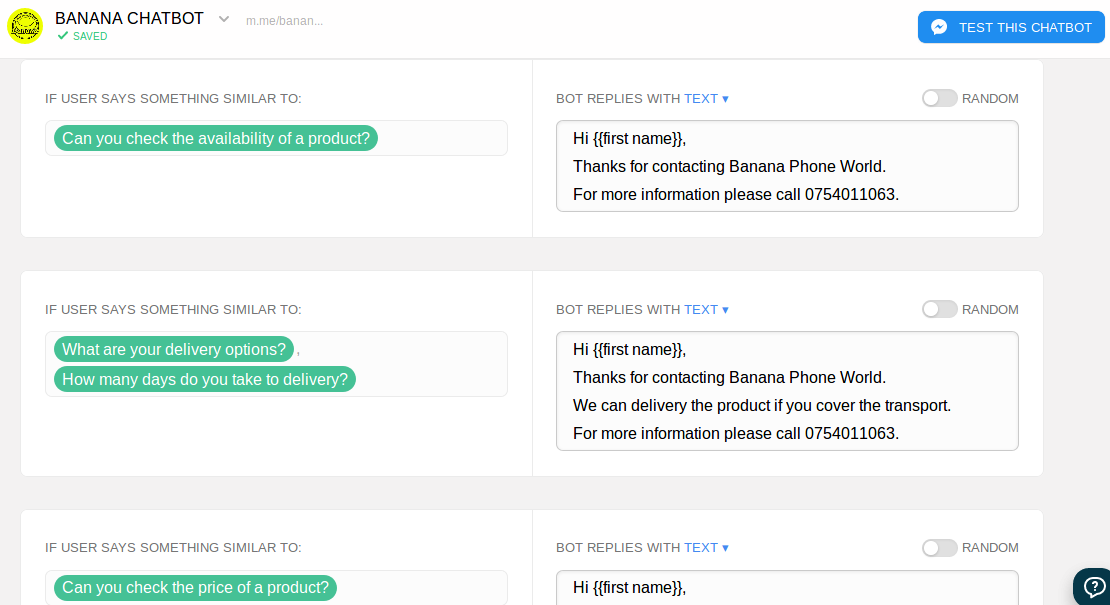
\includegraphics[scale= 0.4]{img/chatfuel.png}
	\caption{Showing the conversation flow }
	\label{fig:symbols}
\end{center}
\end{figure}

\end{itemize}

\section{Phone Repair}

\subsection{Mobile Phone Repairing Tools and Equipment}
During my internship at BPW my supervisor introduced me to their phone technician who really exposed me to alot of experiences concerning both phone hardware and software.
There many tools used in mobile phone repairing but below some of the tools that I used\cite{phone}


\begin{itemize}
\item[1.] \textbf{Soldering Iron:} Used for soldering.
\begin{figure}[h!]
\begin{raggedright}
	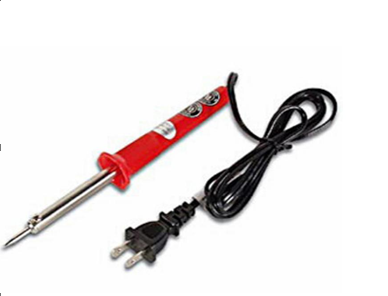
\includegraphics[scale=0.5]{img/solder.PNG}
	\caption{Soldering Iron}
	\label{fig:symbols}
\end{raggedright}
\end{figure}

\item[2.] \textbf{Multimeter:} To check PCB track and electronic Components.
\begin{figure}[h!]
\begin{raggedright}
	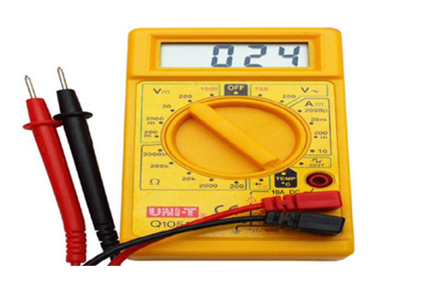
\includegraphics[scale=0.5]{img/multimeter.PNG}
	\caption{Multimeter}
	\label{fig:symbols}
\end{raggedright}
\end{figure}
\begin{figure}[h!]
\begin{center}
	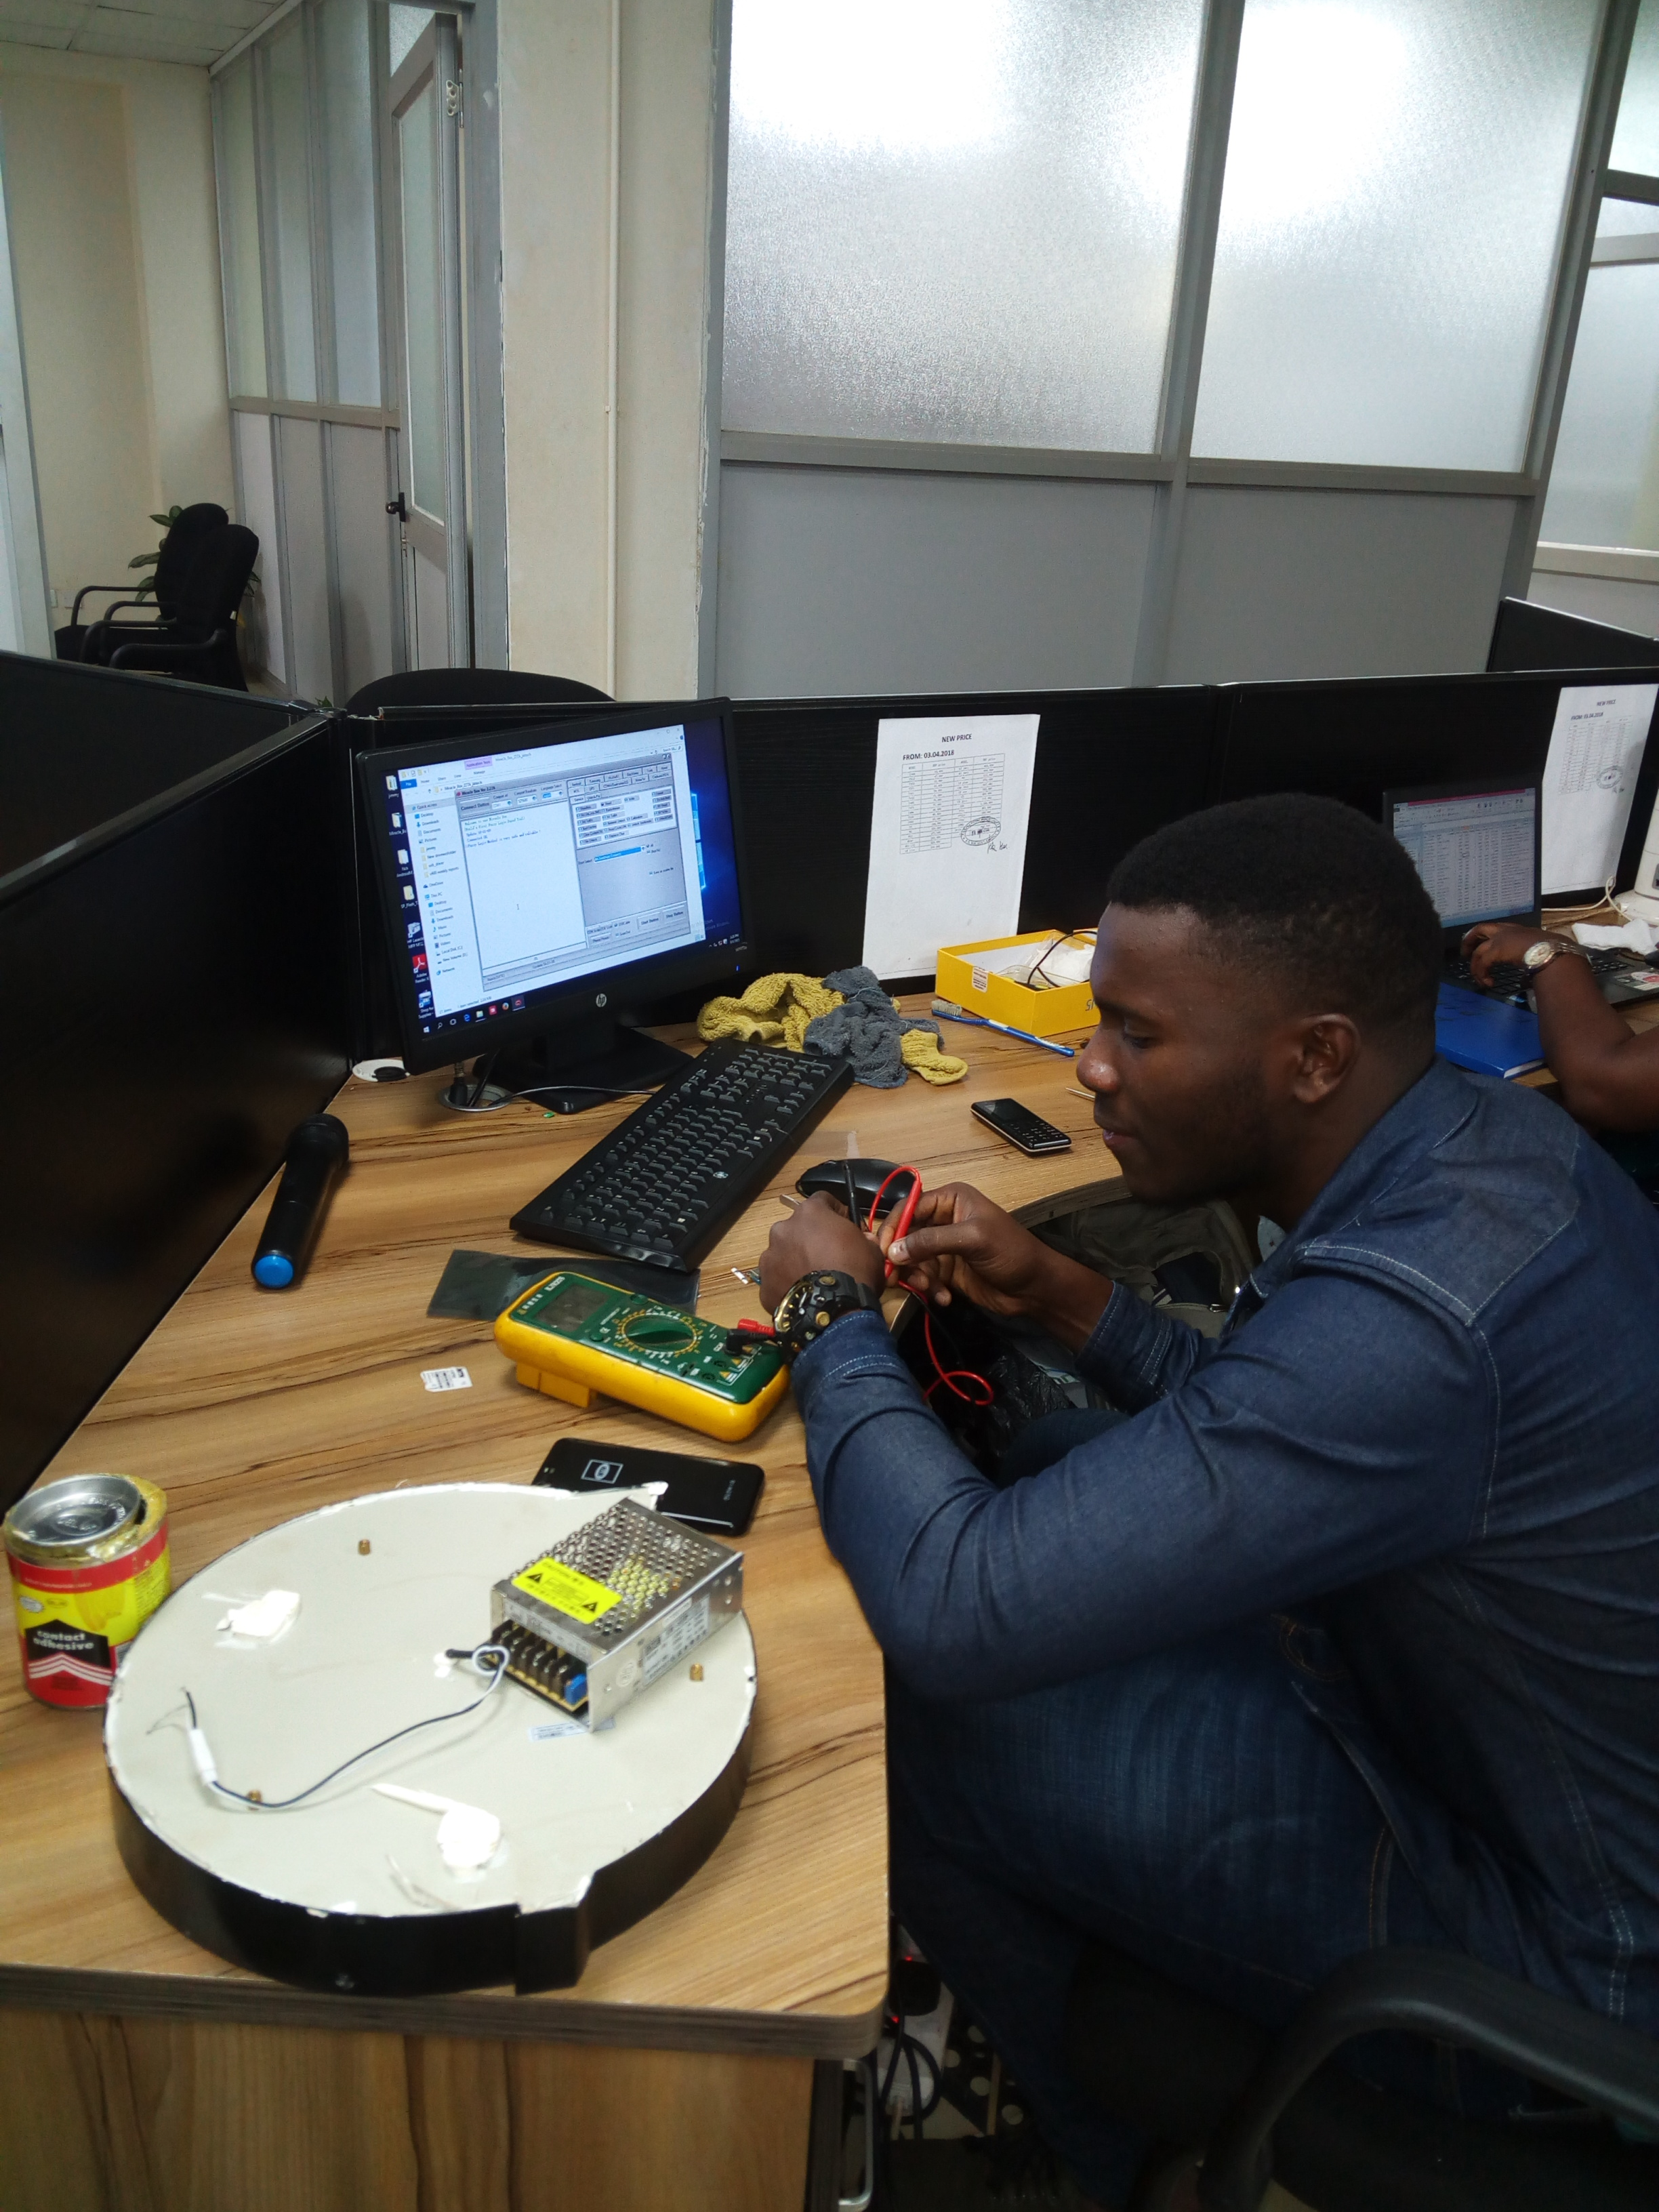
\includegraphics[scale= 0.1]{img/meter.jpg}
	\caption{Me using the multimeter }
	\label{fig:symbols}
\end{center}
\end{figure}


\newpage
\item[3.] \textbf{Screwdriver:} Used to Remove and Tighten Screws from Mobile Phone.
\begin{figure}[h!]
\begin{raggedright}
	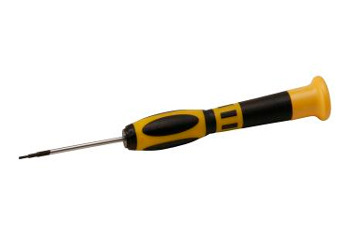
\includegraphics[scale=0.5]{img/screw.PNG}
	\caption{Screw Driver}
	\label{fig:symbols}
\end{raggedright}
\end{figure}

\item[4.] \textbf{Paste Flux:} Used While Soldering.
\begin{figure}[h!]
\begin{raggedright}
	
\includegraphics[scale=0.5]{img/paste.jpg}
	\caption{Screw Driver}
	\label{fig:symbols}
\end{raggedright}
\end{figure}

\end{itemize}

\subsection{Identification of PCB}
The most important part of the phone is the PCB(Printed Circuit Board) which is like the motherboard in the PC so we had to first name the different parts on the PCB and the common faults they normally have.\\
\begin{figure}[h!]
\begin{center}
	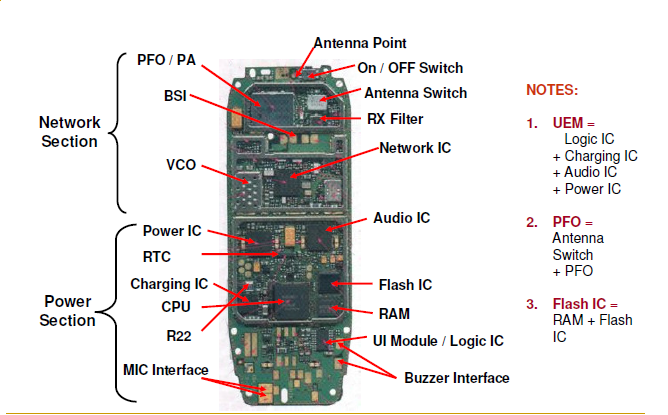
\includegraphics[scale=0.9]{img/PCB.PNG}
	\caption{Printed Circuit Board.}
	\label{fig:symbols}
\end{center}
\end{figure}
\subsubsection{Definition of different Parts of the PCB}
\begin{itemize}
\item[1.] \textbf{Antenna Switch:} It is found in the Network Section of a Mobile Phone and is made up of metal and non-metal. In GSM sets it is found in white colour and in CDMA sets it is found in golden metal.\\ 
\textbf{Function:} It searches network and passes forward after tuning.\\
\textbf{Fault:} If the Anteena Switch is faulty then there will be no network in the mobile phone.

\item[2.] \textbf{P.F.O:} It is found near the Anteena Switch in the Network Section of a Mobile Phone. It is also called P.A (Power Amplifier) and Band Pass Filter.\\
\textbf{Function:} It filters and amplifies network frequency and selects the home network.\\
\textbf{Fault:} If the PFO is faulty then there will be no network in the mobile phone. If it gets short then the mobile phone will get dead.

\item[3.] \textbf{RF IC / Hager / Network IC:} It is found near the PFO in the Network Section of a Mobile Phone. It is also called RF signal processor.\\
\textbf{Function:} It works as transmitter and receiver of audio and radio waves according to the instruction from the CPU.\\
\textbf{Fault:} If the RF IC is faulty then there will be problem with network in the mobile phone. Sometimes mobile phone can even get dead.

\item[4.] \textbf{26 MHz Crystal Oscillator:} It is found near the PFO in the Network Section of a Mobile Phone. It is also called Network Crystal. It is made up of metal.\\
\textbf{Function:} It creates frequency during outgoing calls.\\
\textbf{Fault:} If this crystal is faulty then there will be no outgoing call and no network in the mobile phone.

\item[5.] \textbf{VCO:} It is found near the Network IC in the Network Section of a Mobile Phone.\\
\textbf{Function:} It sends time, date and voltage to the RF IC / Hager and the CPU. It also creates frequency after taking command from the CPU.\\
\textbf{Fault:} If it is faulty then there will be no network in the mobile phone and it will display “Call End” or “Call Failed”.

\item[6.] \textbf{RX Filter:} It is found in the Network Section of a Mobile Phone.\\
\textbf{Function:} It filters frequency during incoming calls.\\
\textbf{Fault:} If it is faulty then there will network problem during incoming
calls.

\item[7.] \textbf{TX Filter:} It is found in the Network Section of a Mobile Phone.\\
\textbf{Function:} It filters frequency during outgoing calls.\\
\textbf{Fault:} If it is faulty then there will network problem during outgoing calls.

\item[8.] \textbf{ROM:} It is found in the Power Section of a Mobile Phone.\\
\textbf{Function:} It loads current operating program in a Mobile Phone.\\
\textbf{Fault:} If ROM is faulty then there will software problem in the mobile phone and the set will get dead.

\item[9.] \textbf{RAM:} It is found in the Power Section of a Mobile Phone.\\
\textbf{Function:} It sends and receives commands of the operating program in a mobile phone.\\
\textbf{Fault:} If RAM is faulty then there will be software problem in the mobile phone and it will get frequently get hanged and the set can even get dead.

\item[10.] \textbf{Flash IC:} It is found in the Power Section of a Mobile Phone. It is also called EEPROM IC, Memory IC, RAM IC and ROM IC.\\
\textbf{Function:} Software of the mobile phone is installed in the Flash IC.
\textbf{Fault:} If Flash IC is faulty then the mobile phone will not work properly and it can even get dead.

\item[11.] \textbf{Power IC:} It is found in the Power Section of a Mobile Phone. There are many small components mainly capacitor around this IC. RTC is near the Power IC.\\
\textbf{Function:} It takes power from the battery and supplies to all other parts of a mobile phone.\\
\textbf{Fault:} If Power IC is faulty then the set will get dead.

\item[12.] \textbf{Charging IC:} It is found in the Power Section near R22.\\
\textbf{Function:} It takes current from the charger and charge the battery.\\
\textbf{Fault:} If Charging IC is faulty then the set will not get charged. If theCharging IC is short then the set will get dead.

\item[13.] \textbf{RTC (Simple Silicon Crystal):} It is found in the Power Section near Power IC. It is made up of either metal or non-metal. It is of long shape.\\
\textbf{Function:} It helps to run the date and time in a mobile phone.\\
\textbf{Fault:} If RTC is faulty then there will be no date or time in the mobile phone and the set can even get dead.

\item[14.] \textbf{CPU:} It is found in the Power Section. It is also called MAD IC, RAP IC and UPP. It is the largest IC on the PCB of a Mobile Phone and it looks different from all other ICs.\\
\textbf{Function:} It controls all sections of a mobile phone.\\
\textbf{Fault:} If CPU is faulty then the mobile phone will get dead.

\item[15.] \textbf{Logic IC / UI IC:} It is found in any section of a mobile phone. It has 20 pins or legs. It is also called UI IC and Interface IC.\\
\textbf{Function:} It controls Ringer, Vibrator and LED of a mobile phone.\\
\textbf{Fault:} If Logic IC / UI IC is faulty then Ringer, Vibrator and LED of mobile phone will nor work properly.

\item[16.] \textbf{Audio IC:} It is found in Power Section of a mobile phone. It is alsocalled Cobba IC and Melody IC.\\
\textbf{Function:} It controls Speaker and Microphone of a mobile phone.
\textbf{Fault:} If Audio IC is faulty then Speaker and Microphone of a mobile phone will not work and the set can even get dead.

\end{itemize}

\subsection{Common phone Faults and solutions}
\begin{itemize}
\item[1.] \textbf{Ringer:} Type of component that rings or plays loud sound is called Ringer. It is also called by several other names like – I.H.F Speaker, Buzzer, Melody etc.
\begin{table}[!ht]
\centering
\begin{tabular}{|p{2.5in}|p{3.5in}|}
\hline
\textbf{Faults} & \textbf{Possible Soultions} \\ \hline
Ringer not working & Check Ringer Settings in Mobile Phone. Check Ringer Volume and Silent Mode.\\ 
Less sound from the Ringer & Open Mobile Phone and Clean Ringer Point and Ringer Connector. \\ Sound coming from Ringer but with interruption & Check Ringer by Keeping the Multimeter in Buzzer Mode. Value must be 8-10 Ohm. If theValue is not between 8-10 Ohm then change the Ringer. \\ 
Sound not clear & Check Track of Ringer Section. Do Jumper Wherever required \\
\hline
\end{tabular}
\caption{Faults \& Solutions of the Ringer.}
\end{table}

\item[2.] \textbf{Vibrator:} Type of component that vibrates. It is also called Motor.Vibrator is controlled by Logic IC or Power IC.
\begin{table}[!ht]
\centering
\begin{tabular}{|p{2.5in}|p{3.5in}|}
\hline
\textbf{Faults} & \textbf{Possible Soultions} \\ \hline
Vibrator not working & Check Vibrator Settings in Mobile Phone. Check if Vibrator is ON or OFF.\\ 
Vibration with interruption & Open Mobile Phone and Clean Vibrator Tips Connector. \\ 
Vibration Hangs & Check Vibrator by Keeping the Multimeter in Buzzer Mode. Value must be 8-16 Ohm. If the Value is not between 8-16 Ohm then change the Vibrator / Motor.\\ 
                & Check Track of Vibrator Section. Do Jumper Wherever required.\\
\hline
\end{tabular}
\caption{Faults \& Solutions of the Vibrator.}
\end{table}

\item[3.] \textbf{Light:} Type of component that generates light in the Mobile Phone. These are generally LED or Light Emitting Diode.
\begin{table}[!ht]
\centering
\begin{tabular}{|p{2.5in}|p{3.5in}|}
\hline
\textbf{Faults} & \textbf{Possible Soultions} \\ \hline
No Light & Check Light Settings.\\ 
Light in only Keypad or Display & Keep Multimeter in Buzzer Mode and Check LED. If LED is Good then it will Glow.If LED is Faulty then it will Not Glow. \\ 
Some lights not working & Change LED or Jumper.\\ 
                & Check Boosting Coil and Change if Required.\\
                & Change Display and Check.\\
\hline
\end{tabular}
\caption{Faults \& Solutions of the LED.}
\end{table}

\newpage
\item[4.] \textbf{Earpiece:} Type of component that helps to listen to sound during phone call. It is also called Speaker or Ear Speaker. Earpiece is controlled by Audio IC or Power IC (UEM).
\begin{table}[!ht]
\centering
\begin{tabular}{|p{2.5in}|p{3.5in}|}
\hline
\textbf{Faults} & \textbf{Possible Soultions} \\ \hline
No sound during phone call & Check Speaker Volume during Phone Call.\\ 
Less sound during phone call & Check Earpiece / Speaker by Keeping the Multimeter in Buzzer Mode. Value must be 25-35 Ohm. If the Value is not between 25-35 Ohm then change the Earpiece / Speaker.
Check Track of Earpiece Section. Do Jumper Wherever required. \\ 
Sound with interruption & Check Track of Earpiece Section. Do Jumper Wherever required.\\ 
                & UEM / Audio IC: Heat, Reball or Change.\\
                & CPU: Heat, Reball or Change.\\
\hline
\end{tabular}
\caption{Faults \& Solutions of the Earpiece.}
\end{table}

\item[5.] \textbf{Screen Touch:} Type of component that helps to operate a mobile phone by touching the screen. Touch Screen is available in different sizes. It normally has 4 Points Namely: - (+), (-), (RX), (TX). Screen Touch is also called PDA. It is controlled by the CPU. In some Mobile Phones there is an Interface IC called PDA IC or Screen Touch IC.
\begin{table}[!ht]
\centering
\begin{tabular}{|p{2.5in}|p{3.5in}|}
\hline
\textbf{Faults} & \textbf{Possible Soultions} \\ \hline
Screen Touch not Working & Check Settings if the Mobile Phone has Both Keypad and Touch Screen.\\ 
Only Half Screen Touch Works & Clean and Resold PDA Tips and PDA Connector. \\ 
One key is pressed and some other key works & Change PDA.\\ 
                & Check Track of the PDA Section and Jumper if Required.\\
                & CPU: Heat, Reball or Change.\\
\hline
\end{tabular}
\caption{Faults \& Solutions of the Screen Touch.}
\end{table}
\newpage
\item[6.] \textbf{Microphone:} Type of component that helps to transmit sound from one mobile phone
to another during phone call.
\begin{table}[!ht]
\centering
\begin{tabular}{|p{2.5in}|p{3.5in}|}
\hline
\textbf{Faults} & \textbf{Possible Soultions} \\ \hline
No sound or Less Sound during phone call & Check Microphone settings.\\ 
Sound with interruption or Changed sound & Check and clean Microphone Tips and Connector. \\ 
                & Check Microphone by Keeping the Multimeter in Buzzer Mode. Value must be 600-1800
Ohm. If the Value is not between 600-1800 Ohm then change the Microphone.\\ 
        
\hline
\end{tabular}
\caption{Faults \& Solutions of the Microphone.}
\end{table}

\item[7.] \textbf{Headphone:} Type of component that does the job of Mic and Speaker separately.
When we insert Headphone, then Speaker and Microphone of the Mobile Phone Gets Disconnected. Headphone is controlled by C.P.U.
\begin{table}[!ht]
\centering
\begin{tabular}{|p{2.5in}|p{3.5in}|}
\hline
\textbf{Faults} & \textbf{Possible Soultions} \\ \hline
No sound from Headphone or sound from only one side of the Headphone & Change the Headphone and Check.\\ 
Sound does no go from the Mic of the Headphone &  Clean Headphone Jack and Connector.\\ 
                & Resolder or Change the Headphone Connector.\\ 
                & Check Track of Headphone Section. Do Jumper Wherever required. \\
\hline
\end{tabular}
\caption{Faults \& Solutions of the Headphone.}
\end{table}

\end{itemize}

\section{Computer Hardware, Software and IT Maintenance}
During my training​ I worked on a number of internal components of a computer like ​mother board, power supply unit, RAM, Hard Disk Drive, CDROM, Floppy drive, CPU, Cable connectors, processor fan, external device jacks like VGA, USB, parallel \& serial ports.​ And I was able to repair some computers (System Units and Laptops) which had a problem and servicing and maintenance and software installations.
\subsection{Servicing computers and maintenance}
Computer servicing and maintenance is the physically cleaning of the interior a​nd  ​exterior of a computer, including the removal of dust and debris from cooling fans, power supplies, and other hardware components, performing diagnostic testing, and making repairs, the detection and removal of computer viruses, update software, install firewalls and security programs, upgrade computer memory, or connect and configure Internet and network connections. During servicing and maintenance a number of tools are used and these include: \\ \\
\textbf{Tools used during servicing and maintenance.} \\ 
\begin{itemize}
\item Electrostatic discharge (ESD) protection kit, including wrist strap and mat 
\item Electric screwdriver.
\item Flashlight
\item Wire cutter or stripper
\item Cleaning swabs, canned air (dust blower), and contact cleaner chemicals
\item Data transfer cables and adapters
\item Diagnostics software
\item Markers, pens, and notepads
\item Spare screws, jumpers, standoffs

\end{itemize}
\textbf{Steps taken during Hardware servicing and maintenance} \\
\begin{itemize}
\item[Step 1-]Before opening the outer case, first unplug the PC if it’s in power.
\item[Step 2-]Then Ground yourself before you touch anything inside to avoid destroying your circuitry with a static charge. If you don't have a grounding wrist strap, you can ground yourself by touching any of various household objects. 
\item[Step 3-]Then use a blower to all the dust in the computer. Mainly on components like the fans, heat sinks, in the corners of the casing, video cards, ATX cable adapters, on the board and other parts. 
\item[Step 4-]Use antistatic wipes to remove the remaining dust from inside the case. Avoid touching any circuit­board surfaces.
\item[Step 5-]Check the expansion slots, unplug them clean the with a brush and plug them back well. After servicing the hardware parts there is need to do software services to maximum computer performance so the next thing to do is perform software maintenance. 
\end{itemize}
\textbf{What was done during software maintenance and servicing computer performance optimization }\\
\begin{itemize}
\item Scanning all computer file and removing virus infections. Before you start on any maintenance program, the first thing you need to do is make sure that you have a clean and healthy computer 
\item Test your hard drive for errors.
\item Remove Unwanted Applications, Ad-ons and Toolbars.
\item Prevent Unnecessary Applications and Services from Loading on Start­up. By disabling them if you don’t want to remove them.
\item Clean up Temp Files this helps to delete unnecessary files – This was done using Windows Disk Clean up utility.
\item Performed drive fragmentation using the Windows Defrag utility.
\item Scan File System for Errors​ –​ for this I used the System File Checker which scans the hard drive for corrupt or missing system files and attempts to replace them.
\end{itemize}

\subsubsection{Software installation and updates}
Computer software or simply software is any set of machine-readable instructions that directs a computer's processor to perform specific operations. There mainly two types of softwares and these include:\\ \\
\textbf{Application software}\\
Application software is the one which uses the computer system to perform special functions or provide entertainment functions beyond the basic operation of the computer itself. \\
\textbf{System software}\\
This is software designed to directly operate the computer hardware, to provide basic functionality needed by users and other software, and to provide a platform for running application software. System software includes: \\
\textbf{Operating systems (OS)}\\
 OS are essential collections of software that manage resources and provides common services for other software that runs "on top" of them. The OS is composed of some core parts such as:\\
 \begin{itemize}
 \item Supervisory programs.
 \item Boot loaders. 
 \item Shells. 
 \item Window systems.
 \end{itemize}
In practice, an operating system comes bundled with additional software (including application software) so that a user can potentially do some work with a computer that only has an operating system. E.g. windows 10, 7, 8, Linux, window XP\\
\textbf{Device drivers}\\
These are software’s which operate or control a particular type of device that is attached to a computer. A driver provides a software interface to hardware devices, enabling operating systems and other computer programs to access hardware functions without needing to know precise details of the hardware being used. \\
Drivers interface with a number of hardware devices. \\
\begin{itemize}
\item printers.
\item video adapter.
\item Network cards.
\item Sound cards.
\item Computer storage devices such as hard disk, CD­ROM, and floppy disk buses.
\item Implementing support for different file systems.
\item Image scanners.
\item Digital cameras. 
\end{itemize}
\textbf{Utilities}
These are either applications or computer programs designed to assist users in maintenance and care of their computers. E.g. registry cleaners, disk defragmenters.\\
\textbf{Malicious software}\\
"Malware" is short form for “malicious software” - computer programs designed to infiltrate and damage computers without the users consent. “Malware” is the general term covering all the different types of threats to your computer safety such as viruses, spyware, worms, trojans, rootkits and so on. 

\subsubsection{What is done before installing software?}
The first thing to do before installing any software is to check System Requirements of your computer whether it meets the minimum system requirements for that product/​​software.  And if you are going to install an operating system on a computer being used first backup all the data to avoid any data loss. \\
Install all system updates and reboot your computer. The final step before beginning installation is to exit all applications that are currently running on your system.

\begin{table}
\centering
\begin{tabular}{|l|p{4.5in}|} % 3 cols (left, ctr, right); vert. lines
% draw horizontal line
\hline
Step 1 & Insert the Windows DVD into your computer's DVD­ROM drive, and restart the computer. Windows  Setup should start automatically. If Setup does not start automatically, ensure that your computer is configured to boot from the DVD drive. \\
\hline
Step 2 & In the next dialog box, you are prompted to start the installation. Click Install Now to begin the installation. This produces a screen that tells you that Setup is starting.  \\
\hline
Step 3 & In the Software License Terms dialog box, ensure that you read and understand the End User Licensing Agreement (EULA). Then select the I Accept the License Terms option and click Next to continue. \\
\hline
Step 4  & Select the Type of Installation You Want. You can select only the Custom (Advanced) option because you're performing a new installation on a blank hard disk. Click Custom (Advanced) to continue. \\
\hline
Step 5 & You choose the partition on which You Want to Install Windows, then click Next.Then the Installing Windows dialog box appears and gives you an updated status of the upgrade process. During this process the computer restarts a couple of times, before the restart, a warning appears.  \\
\hline
Step 6 & After completing the installation, Windows 7 asks you to provide a username and a computer name. After providing this information, click Next to continue.\\
\hline
Step 7 & The next step is to activate windows. Get the key on the cover and type it in the space. 
And lastly make the necessary updates, set the time zone and the location then restart the computer. \\

\hline
\end{tabular}
\caption{Steps for the installation of Windows.}
\end{table}

\section{Projects that I worked due to internship connections}
During my internship, my field supervisor connected me with different people so in that process I got freelance projects that I also worked on which included:
\medskip
\begin{itemize}
\item[1.]\textbf{Web deveploment:} There is a NGO called Mash Child Hope For Africa which is just starting and I am developing for them there website which is still under development up to date.
\item[2.] \textbf{SEO:} I did search engine optimisation for a love spell company based in South Africa and also a company based here in Uganda called \textbf{Katrax Bestway Limited}.
\item[3.] \textbf{Google Forms:} An employee of the company that was working as the social media supervisor had to make a daily report on how many people have liked our facebook page with the influence of our sale representatives from the different shops so I advised him to use google forms but he didnot know about them I helped him design the form and made his work more.  
\end{itemize}
\chapter{Discussion of Experiences}

\section{New knowledge and skills gained in each of the duties and responsibilities}
\subsection{Duties and Responsibilities}
During the internship period, my field supervisor did not assign individual duties and responsibilities, but rather I was required to work with them as they did their daily tasks. My mandate was to have a positive attitude towards the training and show respect to my supervisor and other people we worked with. Therefore, my duty was to work willingly and adhere to tasks I was assigned to do. \\
The following are the main duties and responsibilities that I undertook during the field at BPW.\\
\textbf{End User Support:} I offered end user support on two systems of the company which included:
\begin{itemize}
\item[1.] \textbf{OCMS-BIM:} It is used in stock taking.
\item[2.] \textbf{Egatee:} It is used in e-sales.
\end{itemize}
\textbf{Digital Marketing:} I developed a messenger chatbot for the company as I was instructed by my supervisor which really worked well for BPW because it led to an increase in the sales and inquiries people were making through their facebook fanspage.\\ \\
\textbf{Software installations Installation:} I installed and configured software programs on both Linux and Windows platforms on the employees' computers at BPW.\\
\subsection{New knowledge and skills}
In the internship I accumulated a lot of knowledge and skills during the field attachment. Each of the duties and responsibilities as listed in section 3.1.1 empowered and greatly impacted on my career.\\
In each of the areas trained in, I was able acquire more skills and add on my experience like in installing softwares, anti­viruses, drivers, doing computer maintenance and repair I was able to work on numbers of computers, troubleshooting hardware and others.  
In the area of ethics and conduct, I was able to see and observe the working environment and how people behave and interact. I learnt a lot to do with interpersonal skills, good conduct and organizational culture. 

\section{Most interesting experiences}
During this Field Attachment period, I really enjoyed the experience of working at BPW
including  the  comfortable  working  atmosphere, the friendly relationship among the staff exhibited. Out of all these interesting moments, four extremely interesting experiences are highlighted below.
\subsection{Exhibition of the Infinix Note 5}
One of the very interesting experiences during this internship period was when 
Transsion Holdings officially unveiled the anticipated Infinix Note 5 at a media event held at the Hotel Triangle, in Kampala. The launch of the phablet follows the global launch that was held in Dubai over the weekend. \\
The Infinix Note 5 becomes the third (3rd) phablet Transsion Holdings under Infinix has launched this year. Following the success of the Infinix S3 and the Infinix Hot 6 and Hot 6 Pro which were launched in March and June respectively.

\begin{figure}[h!]
\begin{center}
	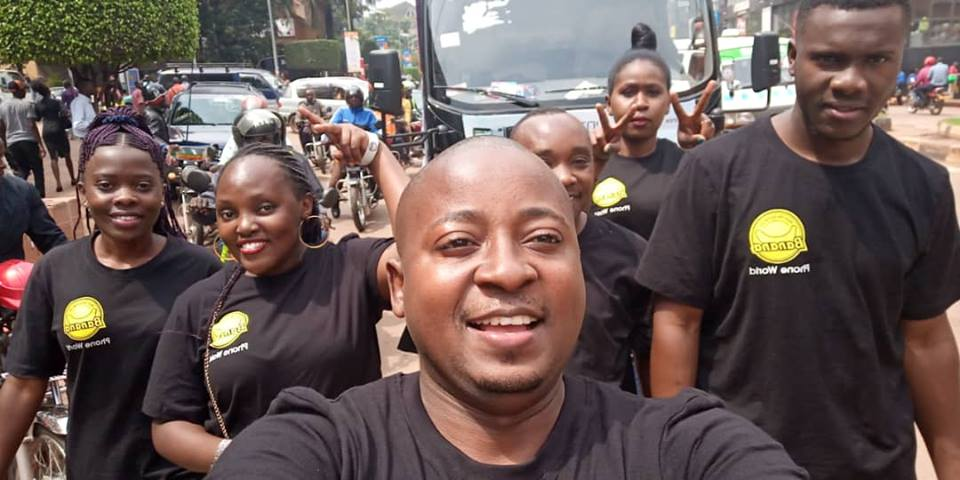
\includegraphics[scale=0.4]{img/klaus.jpg}
	\caption{Me at the extreme right during the exhibition.}
	\label{fig:symbols}
\end{center}
\end{figure}
\newpage
\subsection{Cloning of the Hard Disk}
\noindent Cloning of Hard Disk to install Windows and Ubuntu onto computers whereby
we installed everything at once without need to install application software,
everything was already installed, it was like copying the other Hard Disk onto
the computers.


\section{Relatedness of University's programmes to the Field of work}
Bachelor of Science in Computer Science program at Makerere University provides
professionals with theoretical and practical skills in the IT sector with the aim of
impacting knowledge and skills in fields such as networking, system Administration,
web designing and security management.\\ \\
During my two years I have studied quite a number of course units such as Computer
Literacy, Communication Skills and Operating System to mention but a few.All these course units are clearly related to duties I engaged in while at BPW and they are clearly explained in detail below.
\begin{itemize}
\item[*] Communication Skills was applied in effective speaking and listening skills that were taught at university  during  communications,  meetings  and  presentation sessions.
\item[*] Computer Literacy  skills  such as Microsoft Word, Excel and power point  to  prepare  professionally  looking  and  standard documents at work.
\item[*] Operating Systems was aplied in the windows and linux installation. 

\end{itemize}
These are just a few selected courses showing how the taught university programs are indeed relevant in the field of work. Even other courses not mentioned here, such as those in the field of networking are relevant, only that the intern never undertook tasks in that field during this period.
\section{Challanges faced and how managed}
Just like in any other organization, one is bound to experience a number of problems both at places of work and individual problems. The problems faced were related to work and these included the following.
\begin{itemize}
\item Time management challenged me in that I had to wake up very early to dodge the traffic jam so as I’m always early at my workplace. This proved to be a challenge to me but with time I coupled up with it.
\item I was challenged with the problem of money since this included transport and lunch. At times we were given some research work and this needed me to buy some internet bundles to inject in so as to buy data for my research work. I had my savings and my parents also provided me with some cash.
\item I was challenged with the problem of software incompatibility required to be installed onto the employees' computers. The software I always had required a 64 Bit computer and yet some machines were 32 bit machines.So I had to download some software from the internet which was compatible with those machines.
\end{itemize}
\section{Benefits derived from Field Attachment}
Besides the knowledge and skills talked about, the intership training gave me an opportunity to connect and interact with people in the same profession and people from different parts of the world.
\begin{itemize}
\item I gained a skill of time management and responsiveness of the duties and
activities assigned to me.
\item The training also enabled me to create useful friends who will motivate me in my carrier. I also got opportunity of being exposed to challenges at places of work and how they can be resolved.
\item I gained skills in online marketing and content management at large.
\item I learnt alot about smartphones especially Tecno, Infinix and Itel models.
\end{itemize} 
\section{Career Motivation}
While at BPW, I've been motivated to work harder, be creative and innovative in
different aspects as this would encourage me stay focused since most organizations
need creative IT persons.\\ \\
My internship attachment at BPW also helped me gain more professional skills that aren't gained in lecture rooms. This encouraged me to equip myself with all basic skills and enchance my CV in the future.


\chapter{Conclusion and Recommendations}

\section{Recommendations}
I recommend to allow students engage in internship trainings at every end of the study year this will help students gain more experience, skills and knowledge. Students will also get used to the real working world hence producing competent graduates with enough experience and skills. \\ \\
I also recommend the university to improve on the teaching mode by engaging students more in practical projects rather than waiting for the final year project.

\section{Conclusion}
In conclusion, this training period has been so nice that have been able to practically apply my theory, acquire more knowledge by cooperating with my field supervisor through asking what I don’t know and learn very many things.  \\ \\
And I think this training was worthy it to be done. Thank all staff of Banana Phone World Ltd so much for their support, encouragement, conducive working environment and training because have I gained a lot. \\ \\
I thank the University for such an Arrangement because it’s very useful and also helps to produce practical oriented graduates. The idea of industrial training is very good since students are able to learn a lot of practical work, get exposed to the outside world and potential employers, this helps them after their course to get to appreciate their profession hence get better ethics and an opportunity to put to use their theoretically acquired knowledge into practical things. It was also a great experience being at the training where all that I had seen in books were laid bare and done by me.



% \input{./conclusion.tex}
% \input{./acknow.tex}
% \input{./ref.tex}
%\input{./future-work.tex}

%\bibliographystyle{plain}
%\bibliography{references}

\begin{thebibliography}{999}

  \bibitem{Digital}
  Digital Marketing Made Simple: A Step-by-Step Guide, 'Neil Patel'. [Online].
  Available: \url{https://neilpatel.com/what-is-digital-marketing/}, 
  [Accessed: June 08, 2018].
  
  \bibitem{chatbot}
  Chatbot Development, 'Chatfuel dashboard'. [Online].
  Available: \url{https://dashboard.chatfuel.com/}, 
  [Accessed: June 18, 2018].
  
  
  \bibitem{phone}
	  Mobile Phone Repairing PDF Book Free Tutorial \& Guide, 'Mobile Phone Repairing', January 20,          	  2018. [Online].Available: \url{http://www.mobilecellphonerepairing.com/mobile-phone-repairing-		  pdf-book-free-tutorial-guide.html}, 
  	  [Accessed: July 08, 2018].
  
 
\end{thebibliography}

\chapter{Appendices}
\section{Appendix A: Applications and Systems that I interacted with.}

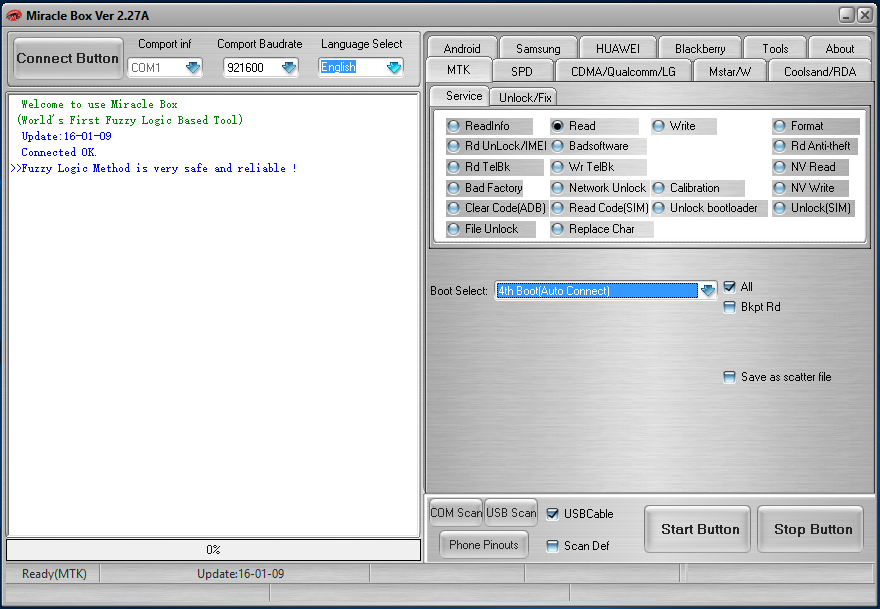
\includegraphics[width=\linewidth]{img/miracle.PNG}
\captionof{figure}{Miracle box that is used in phone software including flashing, read patterns and many others.}
\bigskip

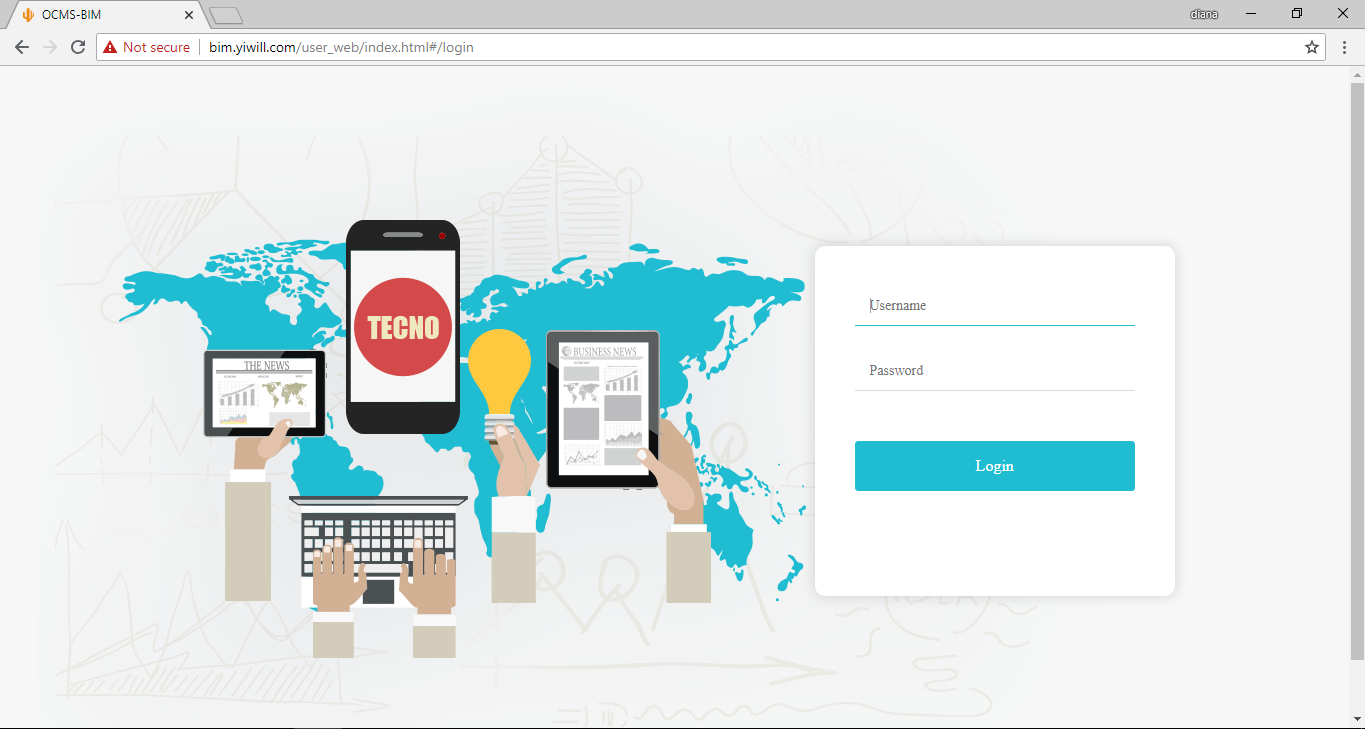
\includegraphics[width=6in]{img/ocmis.PNG}
\captionof{figure}{OCMIS-BIM Login.}
\bigskip
\newpage

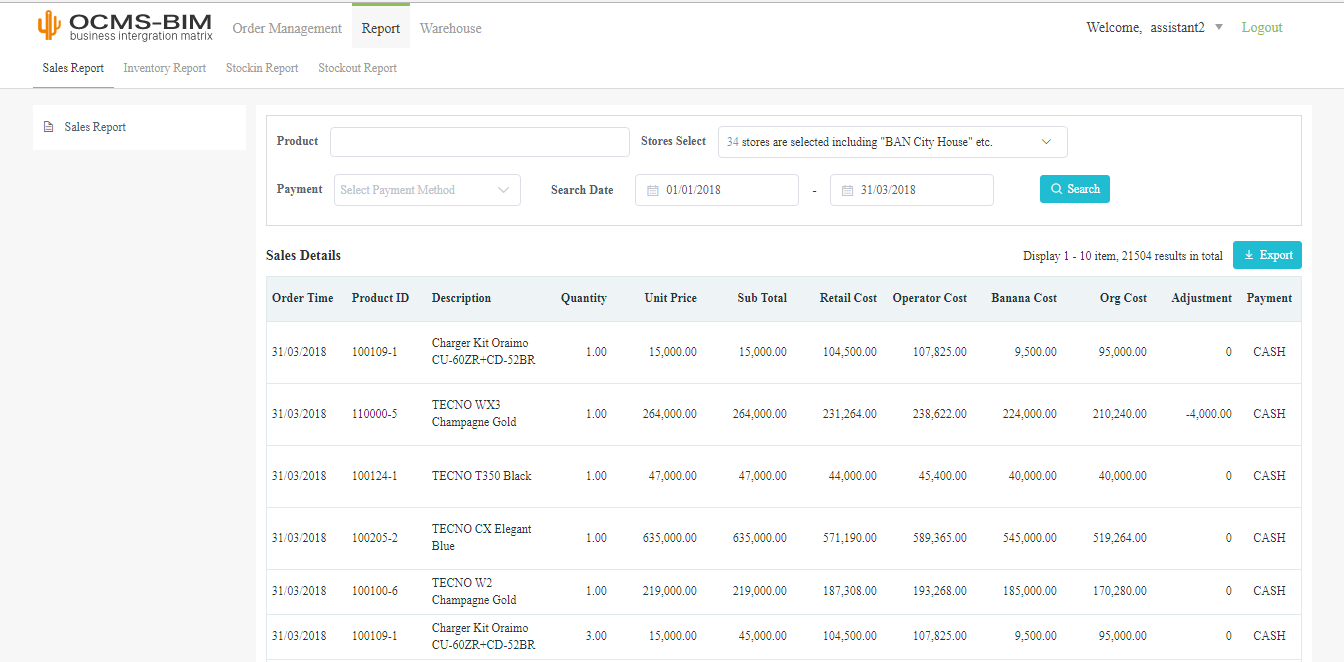
\includegraphics[width=6in]{img/bim.PNG}
\captionof{figure}{OCMIS-BIM system that is used in stock taking.}
\bigskip
\newpage

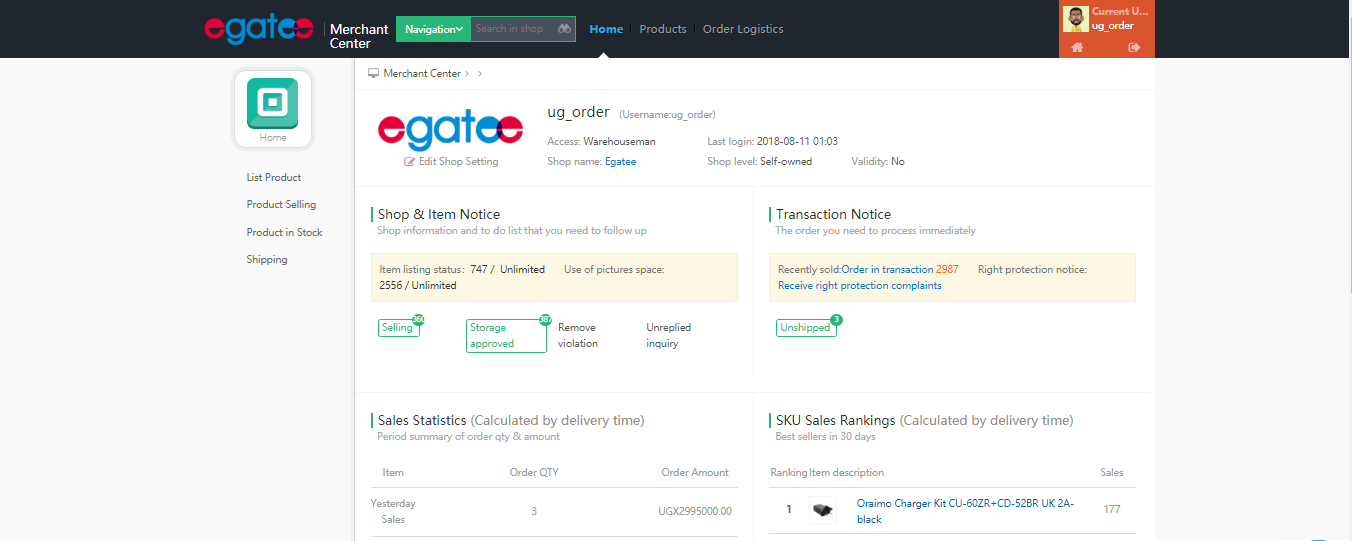
\includegraphics[width=\linewidth]{img/Egatee.PNG}
\captionof{figure}{Egatee web system that is used in the e-sales.}
\bigskip

\centering
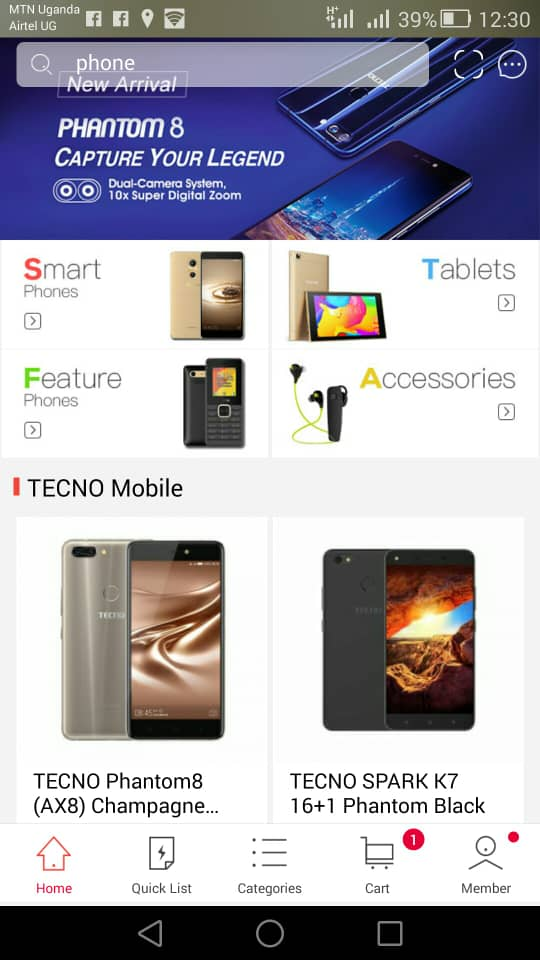
\includegraphics[width=3.5in]{img/Egatee1.jpeg}
\captionof{figure}{Egatee Mobile App that is used by the wholesalers to purchase the products.}
\bigskip

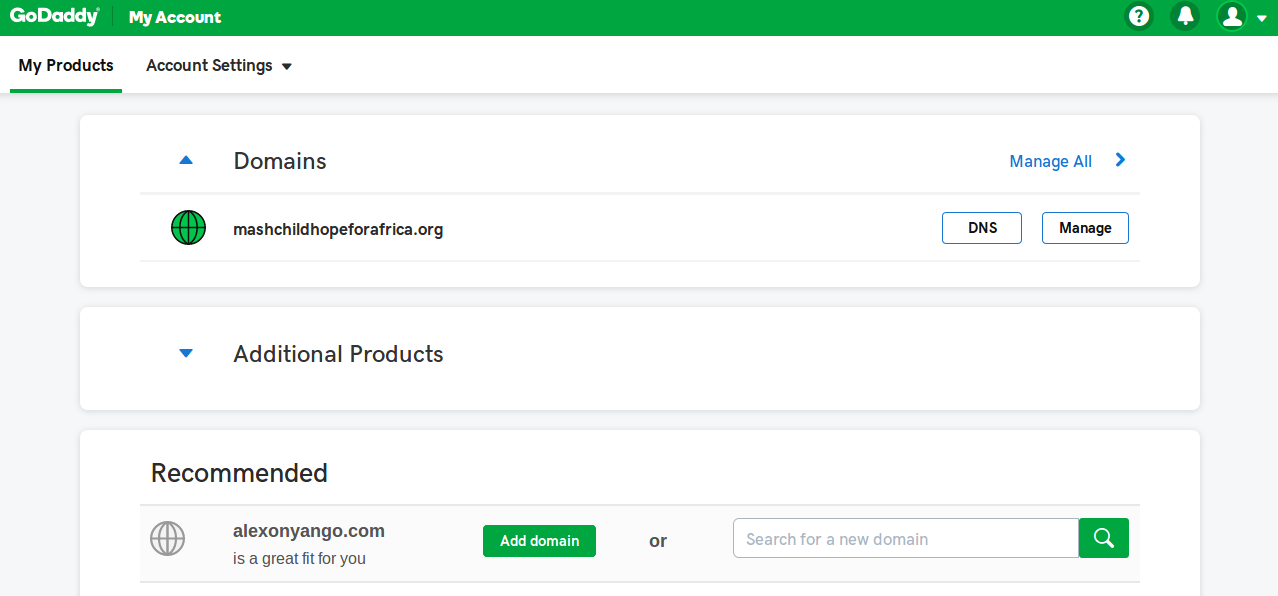
\includegraphics[width=\linewidth]{img/godaddy.png}
\captionof{figure}{Showing the domain of \textbf{mashchildhopeforafrica.org} I purchased from GoDaddy.}
\bigskip
\newpage

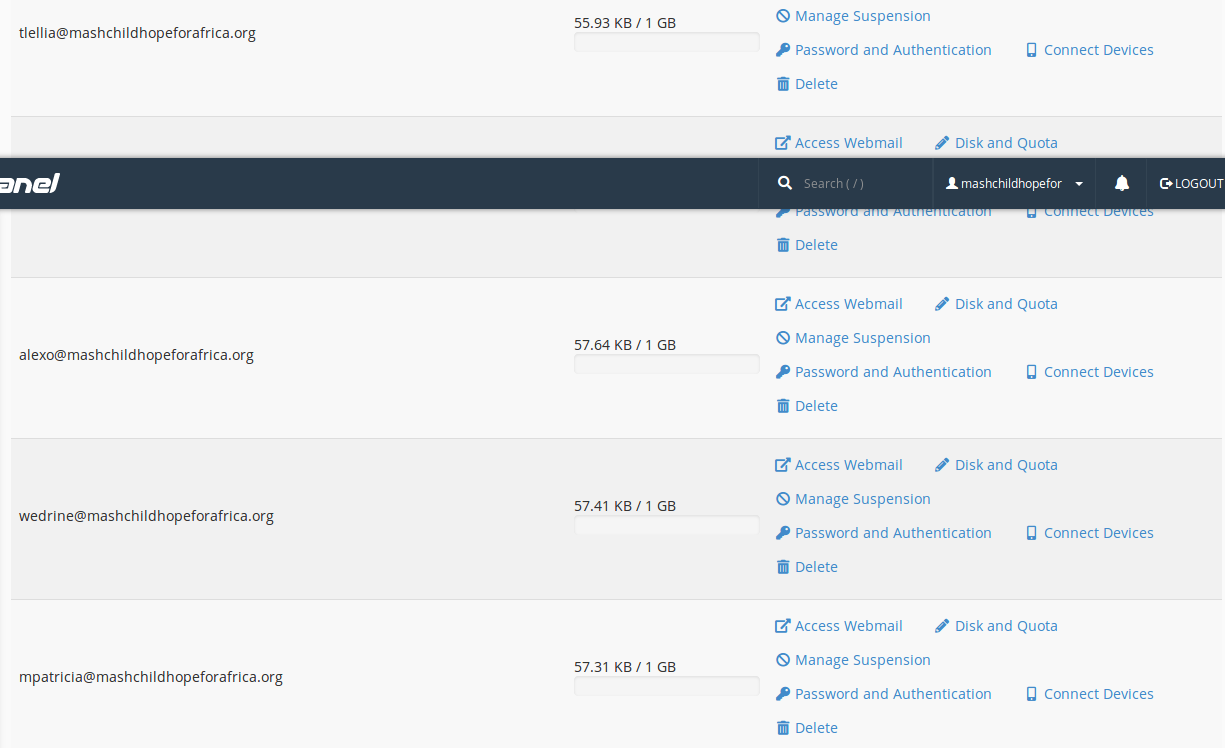
\includegraphics[width=\linewidth]{img/k.png}
\captionof{figure}{Emails I created via Cpanel.}
\bigskip
\newpage

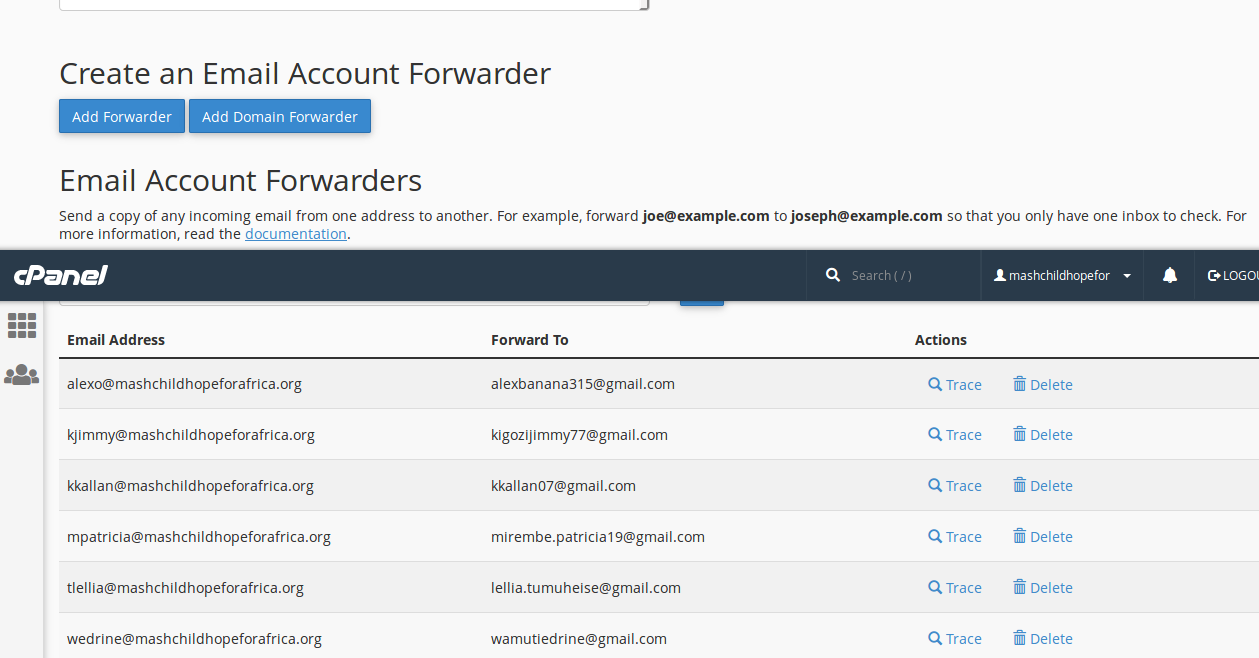
\includegraphics[width=\linewidth]{img/Forwarders.png}
\captionof{figure}{Emails being forwarded to the gmails of the clients.}
\bigskip
\newpage

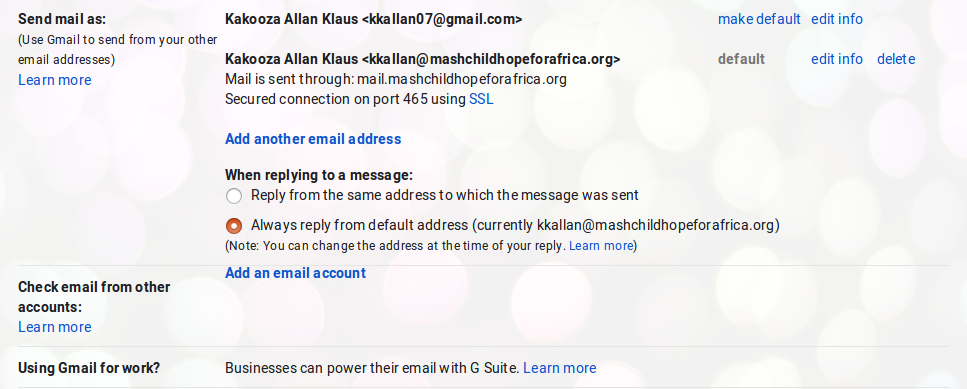
\includegraphics[width=\linewidth]{img/gmail.png}
\captionof{figure}{Configuration of the Gmail to be the default mail server for the \textbf{mashchildhopeforafrica.org}.}
\bigskip
\newpage

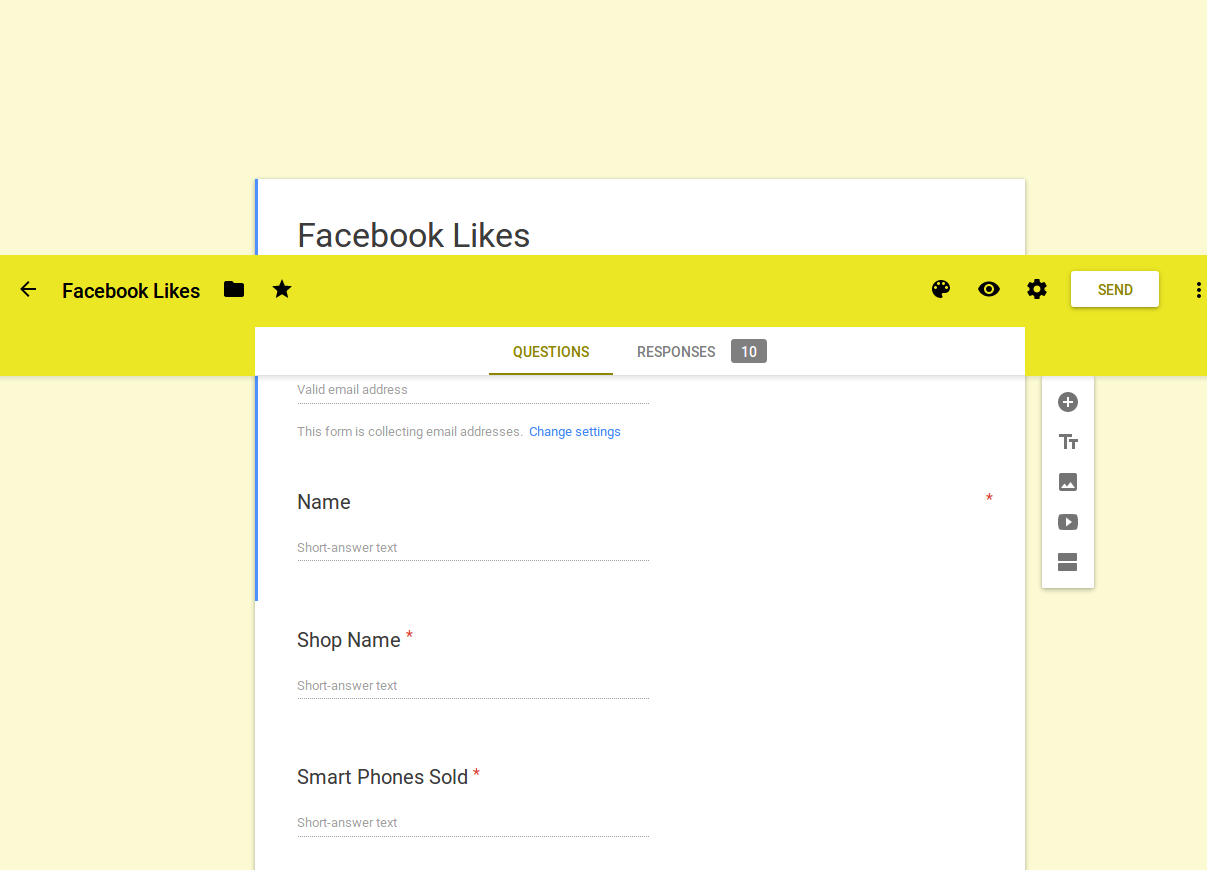
\includegraphics[width=\linewidth]{img/googleforms.png}
\captionof{figure}{The Form I designed using google forms.}
\bigskip

\newpage
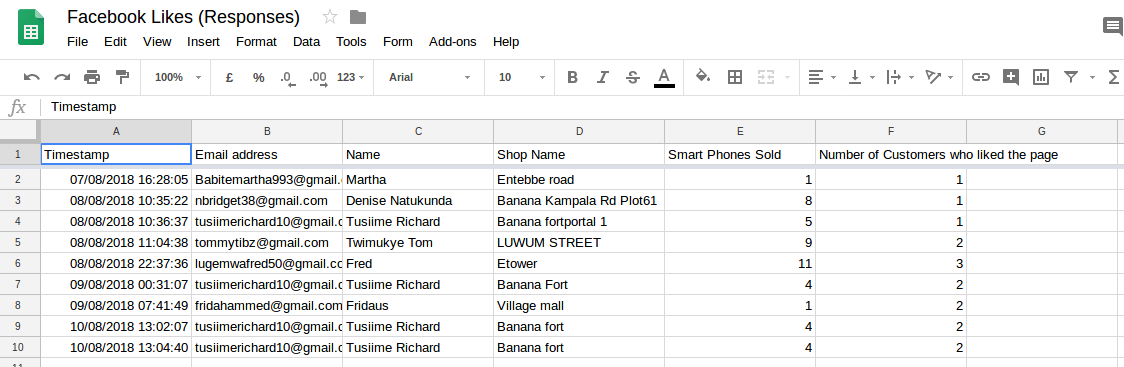
\includegraphics[width=\linewidth]{img/Facebook.png}
\captionof{figure}{The spreadsheet that was linked to the google form.}
\bigskip

\end{document}
